\chapter{Imaginary Matrices in 3D Realspace}

\section{Euler’s Identity as a Collapse Operator}

Imaginary numbers serve as a buffer overflow for when dimensional boundaries are broken by mathematics. \cite{imaginary_meta} Euler’s identity is a perfect example of this:

\[
e^{i\pi} = -1
\]

Euler’s identity inherently describes a rotation of the natural number $e$ into imaginary space---a vector, in some ways, to the imaginary dimension. \cite{imaginary_meta} It acts as a transitional bridge between the potential and the actual, between the unresolved quantum flux and the collapsed, real state\footnote{See Nahin, Paul J., \textit{An Imaginary Tale: The Story of $\sqrt{-1}$}, Princeton University Press, 1998. \cite{imaginary_meta} For further application in physics, consult Arfken, Weber, and Harris, \textit{Mathematical Methods for Physicists}, Elsevier, 2013.}. \cite{imaginary_meta} 

In Measurement Field theory, Euler’s identity is no longer just a mathematical curiosity-it is a \textbf{fundamental description of collapse} itself. \cite{imaginary_meta} The exponential function $e^{ix}$, when rotated by $\pi$, lands precisely at $-1$, signifying the transition from potential (imaginary) to opposition (real, negative). \cite{imaginary_meta} This is the mathematical fingerprint of observation-when imaginary potential is resolved through the act of measurement, it manifests in realspace as coherent structure. \cite{imaginary_meta} The negative real outcome isn't destructive-it is \textbf{stabilizing}. 

Euler’s constant $e$, often regarded as a base for growth or decay, here operates as the \textbf{time-decay factor of unresolved possibility}. The oscillation encoded in $e^{ix}$ defines the phase evolution of a quantum state pre-collapse, and its interaction with $\pi$ -a geometric, circular constant-represents the wrapping of uncollapsed information into definable boundary constraints. \cite{imaginary_meta} 

In this manner, Euler’s identity becomes a \textbf{keystone equation} for collapse modeling: the transition function by which the measurement field filters chaotic potential into structured definition. \cite{imaginary_meta} It encapsulates how finely reality itself can resolve quantum foam into observable states-the mathematical measure of how the universe approximates its own existence from infinite probabilities. \cite{imaginary_meta} 

The number $e$ is resolved by a system of a natural logarithmic value over time, infinitely approaching $\log(n)$, which reflects how definition becomes sharper as collapse density increases. \cite{imaginary_meta} Euler’s constant is not an arbitrary resolution factor-it is the \textbf{quantum scaffold}-the baseline by which collapse coherence and observational force exert their influence on probabilistic systems. \cite{imaginary_meta}

Without Euler’s identity as a grounding principle, the Measurement Field would lack a stable gradient.\cite{imaginary_meta} Its inclusion here is not just theoretical-it is novel. To the best of our knowledge, no prior work has explicitly mapped the functional implications of Euler’s identity into the collapse mechanics of 3D imaginary matrices in realspace. \cite{imaginary_meta}

This approach, as formulated within Measurement Field theory, represents an original expansion into the visual and functional modeling of collapse as a phase resolution process grounded in the exponential framework of imaginary rotation. \cite{imaginary_meta} It is, therefore, among the first formal attempts to tie Euler’s identity directly to physical collapse architecture within a real-imaginary dynamic field. \cite{imaginary_meta} Superposition would never resolve, and the emergence of classical behavior would be impossible. \cite{imaginary_meta} Its presence in the theoretical framework confirms the necessity of imaginary structure in the real evolution of the universe. 

\section{Graphing Imaginary Matrices in Realspace}

To graph an imaginary matrix in realspace, one must construct a mapping between the complex domain and its projection within three-dimensional space. \cite{imaginary_meta}

Imaginary matrices-especially those involving complex eigenvalues-can be visualized by decomposing them into their real and imaginary components and assigning dimensional roles. \cite{imaginary_meta}

Let a complex matrix $M$ be defined such that:

\[
M = A + iB
\]

Where $A$ and $B$ are real-valued matrices of equal dimensions. \cite{imaginary_meta} The mapping to 3D realspace involves treating $A$ as the "classical" structure and $B$ as the oscillatory, rotational, or potential field overlay. \cite{imaginary_meta} These dual components express the physical and pre-physical states of a system respectively. 

To visualize this, one can graph each complex entry $m_{ij} = a_{ij} + ib_{ij}$ as a vector in 3D space:

\[
\vec{v}_{ij} = (i, j, a_{ij}), \quad \text{with color or vector rotation denoting } b_{ij}
\]

Alternative encodings:
\begin{itemize}
    \item \textbf{Real axis}: height or radial distance. \cite{imaginary_meta} 
    \item \textbf{Imaginary axis}: hue, phase rotation, or quiver field. \cite{imaginary_meta} 
    \item \textbf{Magnitude}: opacity or scaling. 
    \item \textbf{Directionality}: rotational spin for encoding complex argument. \cite{imaginary_meta} 
\end{itemize}

This strategy is conceptually aligned with existing practices in quantum state tomography \footnote{See D'Ariano, Paris, and Sacchi, "Quantum Tomography", Advances in Imaging and Electron Physics, Vol. 128 (2003)} and complex systems modeling where phase-space visualization encodes complex amplitudes into real representational planes \footnote{For an overview, consult Cvitanovi\'c et al., "Chaos: Classical and Quantum", Niels Bohr Institute (2016)}. \cite{imaginary_meta} 

It allows us to encode the imaginary dimension as a visual phenomenon without violating the 3D substrate. In essence, we make the invisible visible through coherent mapping. 

\section{Collapse Dynamics and Derivatives}

Let $M : \mathbb{R}^3 \times \mathbb{R} \rightarrow \mathbb{C}$ be a scalar complex field defined over space and time. \cite{imaginary_meta} We define:

\[
M(\vec{x}, t) = A(\vec{x}) + i B(\vec{x}, t)
\]

Where:
\begin{itemize}
    \item $A(\vec{x})$ is the real-valued, time-invariant structural matrix. 
    \item $B(\vec{x}, t)$ is the imaginary-valued, time-dependent potential field undergoing observational collapse. \cite{imaginary_meta} 
\end{itemize}

The total magnitude of the field is:

\[
|M(\vec{x}, t)| = \sqrt{A(\vec{x})^2 + B(\vec{x}, t)^2}
\]

We now derive the temporal and spatial collapse dynamics of the field. \cite{imaginary_meta} 

\paragraph{Time Derivative of Collapse:}

We posit a first-order exponential decay law on $B$:
\[
B(\vec{x}, t) = B_0(\vec{x}) \cdot e^{-\alpha t}
\quad \Rightarrow \quad
\frac{\partial B}{\partial t} = -\alpha B
\]

Thus, the time derivative of the magnitude becomes:
\[
\frac{\partial |M|}{\partial t} = \frac{-\alpha B^2}{\sqrt{A^2 + B^2}}
\]

This expression is nonlinear and approaches zero as $B \rightarrow 0$, representing the completion of collapse. \cite{imaginary_meta} 

\paragraph{Spatial Gradient of Collapse:}

The spatial gradient of the magnitude field is given by:
\[
\nabla |M| = \frac{A \nabla A + B \nabla B}{\sqrt{A^2 + B^2}}
\]

This gradient captures local deformation of the collapse field and serves as a measure of field tension or coherence instability. \cite{imaginary_meta} 

\paragraph{Collapse Tension Norm:}

Define the full collapse pressure tensor norm (a novel construct introduced here, differing from stress-energy tensors or Ricci curvature in general relativity):
\[
\|\nabla |M|\| = \sqrt{ \left( \frac{\partial |M|}{\partial x} \right)^2 + \left( \frac{\partial |M|}{\partial y} \right)^2 + \left( \frac{\partial |M|}{\partial z} \right)^2 }
\]

High values of $\|\nabla |M|\|$ identify transition zones-regions of high informational curvature where collapse is incomplete or actively occurring. \cite{imaginary_meta} 

\begin{theorem}[Collapse Gradient Theorem]
Given the field $M(\vec{x}, t)$ defined as above, the temporal and spatial evolution of observational collapse is defined by:
\[
\frac{\partial |M|}{\partial t} = \frac{-\alpha B^2}{|M|}, \qquad
\|\nabla |M|\| = \left\| \frac{A \nabla A + B \nabla B}{|M|} \right\|
\]
\end{theorem}

These quantities are visualized in Chapter 1 via field plots and quiver representations of local tension, and in later chapters via higher-order tensor decomposition and field phase analysis. \cite{imaginary_meta}

In Collapse Field simulation, the imaginary component may represent the undetermined, oscillatory phase space prior to observation. \cite{imaginary_meta} Thus, the imaginary matrix is not a detached phantom-it is the reservoir of all possible quantum states not yet resolved. \cite{imaginary_meta} It acts as the domain in which chaos is tamed and raw potential transitions into ordered structure. 

\section{Laplacians and Collapse Topology}

To extend our analysis, we apply the Laplace operator to the collapse magnitude field:

\[
\Delta |M| = \nabla \cdot \left( \nabla |M| \right)
\]

Substituting the expanded form:
\[
|M| = \sqrt{A^2 + B^2}, \quad \text{with } B = B_0 e^{-\alpha t}
\]

We compute the Laplacian in Cartesian coordinates as:
\[
\Delta |M| = \frac{\partial^2 |M|}{\partial x^2} + \frac{\partial^2 |M|}{\partial y^2} + \frac{\partial^2 |M|}{\partial z^2}
\]

By differentiating the previously defined magnitude expression:

\[
\frac{\partial^2 |M|}{\partial x^2} =
\frac{
    (A^2 + B^2)\left(A'' + B''\right) + (A A' + B B')^2 - (A A'' + B B'') (A^2 + B^2)
}
{
    (A^2 + B^2)^{3/2}
}
\quad \text{(symbolic form)}
\]

In regions where $B$ dominates, this Laplacian reveals collapse curvature-zones of extreme tension decay or local coherence nucleation. \cite{imaginary_meta} A positive Laplacian indicates field expansion (void formation), while a negative value indicates contraction (collapse compression). \cite{imaginary_meta} 

Thus, $\Delta |M|$ defines the collapse topology curvature, akin to a second-order coherence flow:
\[
\Delta |M| \propto \text{collapse field curvature}
\]

This term will later inform boundary behavior in black hole horizons (Chapter 6), retrocausal reinsertion (Chapter 8), and multibranch structural interference (Chapter 9). \cite{imaginary_meta} 

\begin{theorem}[Collapse Curvature Laplacian]
Given the collapse magnitude field $|M| = \sqrt{A^2 + B^2}$, with $B(t) = B_0 e^{-\alpha t}$, the Laplacian of collapse is:
    
\[
\Delta |M| = \nabla^2 |M| = \frac{\partial^2 |M|}{\partial x^2} + \frac{\partial^2 |M|}{\partial y^2} + \frac{\partial^2 |M|}{\partial z^2}
\]
    
This expression governs the second-order differential geometry of collapse and encodes local field convergence or divergence. \cite{imaginary_meta} It acts as the collapse-field analogue of Ricci curvature in classical general relativity. \cite{imaginary_meta} 
\end{theorem}

\section{Field Action and Lagrangian Formalism}

  \begin{mdframed}[style=collapsebox]

    \textbf{Collapse Field Lagrangian (Measurement Field Action)}
    
    Let the complex collapse field be defined as:
    \[
    M(\vec{x}, t) = A(\vec{x}) + i B(\vec{x}, t)
    \]
    where $A$ is the classical real structure and $B$ is the time-evolving imaginary potential. \cite{imaginary_meta} 
    
    We define the Lagrangian density $\mathcal{L}$ over spacetime as:
    \[
    \mathcal{L} = \frac{1}{2} \left( \partial_\mu M^* \, \partial^\mu M \right) - V(|M|)
    \]
    
    Where:
    \begin{itemize}
      \item $\partial_\mu M$ includes time and spatial derivatives,
      \item $V(|M|)$ is a collapse potential, enforcing classical convergence. \cite{imaginary_meta} 
    \end{itemize}
    
    \textbf{Kinetic Term:}
    \[
    \partial_\mu M^* \, \partial^\mu M = \left| \frac{\partial M}{\partial t} \right|^2 - \left| \nabla M \right|^2
    \]
    
    \textbf{Collapse Potential:}
    \[
    V(|M|) = \frac{1}{2} \alpha^2 B^2
    \]
    
    \textbf{Action Functional:}
    \[
    S[M] = \int \mathcal{L}(M, \partial_\mu M) \, d^4x
    \]
    
    Collapse follows the principle of least action:
    \[
    \frac{\partial \mathcal{L}}{\partial M} - \partial_\mu \left( \frac{\partial \mathcal{L}}{\partial (\partial_\mu M)} \right) = 0
    \]
    
    This yields a nonlinear collapse wave equation driven by decay in $B$ and constrained by spatial coherence. \cite{imaginary_meta} The Measurement Field dynamically resolves into observable reality via the evolution of this action. \cite{imaginary_meta}   

  \end{mdframed}
    

\newpage


\section{Measurement Entropy and Thermodynamic Collapse}

We define a local entropy density $\mathcal{S}(x, t)$ as a functional of the imaginary field component $B(x, t)$:

\[
\mathcal{S}(x, t) = -\eta \cdot B^2(x, t) \cdot \log\left( \frac{B^2(x, t)}{B_0^2(x)} \right)
\]

Where:
\begin{itemize}
  \item $\eta$ is a dimensional scaling constant,
  \item $B_0(x)$ is the initial (maximum) observer-potential at $t = 0$,
  \item $\mathcal{S}(x, t)$ represents the unresolved measurement entropy at spacetime point $(x, t)$. \cite{imaginary_meta} 
\end{itemize}

This formulation is analogous in spirit to the von Neumann entropy $S = -\text{Tr}(\rho \log \rho)$ used in quantum information theory, where the density matrix $\rho$ captures the state of a quantum system. \cite{imaginary_meta} Here, instead of working with a full density matrix, we collapse this to a spatial field-based representation. $B^2(x,t)$ acts as a local probabilistic amplitude analogue, and the entropy quantifies the local uncertainty or informational degeneracy remaining before collapse. \cite{imaginary_meta} 

\paragraph{Total Field Entropy:}
We define the full field entropy as:
\[
S(t) = \int_{\mathbb{R}^3} \mathcal{S}(x, t) \, d^3x
\]

This integral gives the total measurement entropy at time $t$. \cite{imaginary_meta} It is strictly decreasing under exponential decay:

\[
\frac{dS}{dt} = -\eta \cdot \int B(x,t)^2 \left( \alpha + \log \left( \frac{B^2(x,t)}{B_0^2(x)} \right) \cdot \alpha \right) d^3x < 0
\]

\paragraph{Collapse Entropy Law:}
Measurement-field evolution obeys an entropy law analogous to thermodynamic systems:
\[
\frac{dS}{dt} < 0
\quad \text{as } B \rightarrow 0
\]

This formalism reframes collapse as an \textbf{entropy extraction process}. \cite{imaginary_meta} Classical states are those with \textbf{minimal residual measurement entropy}. \cite{imaginary_meta} 

\paragraph{Collapse Completion Criterion:}
Collapse at point $x$ is considered complete when:
\[
\mathcal{S}(x, t) < \epsilon
\quad \text{for some small } \epsilon > 0
\]

indicating that local observer-potential has fully resolved into definitional realspace. \cite{imaginary_meta} 

\subsection*{Collapse as a Statistical Ensemble Process}

The Measurement Field can be interpreted as a dynamic statistical ensemble where $B(x, t)$ represents a field of unresolved microstates. \cite{imaginary_meta} 

At $t = 0$, the imaginary component $B_0(x)$ corresponds to a \textbf{maximally degenerate ensemble}, i.e., many possible microstates. 

Collapse evolves this system toward lower entropy, analogous to the \textbf{statistical narrowing of possible configurations}. \cite{imaginary_meta} 

\paragraph{Partition Functional:}
We define a collapse partition functional:
\[
Z = \int e^{-\beta B^2(x)} \, d^3x
\]

Where:
\begin{itemize}
  \item $\beta = \alpha^{-1}$ plays the role of an \textbf{inverse measurement temperature},
  \item $B^2(x)$ acts as a field-based "energy" term---configurations with high $B$ contribute less to the ensemble. \cite{imaginary_meta} 
\end{itemize}

\paragraph{Collapse Probability Distribution:}
The local probability density of a collapse state $B(x)$ is:
\[
P(x) = \frac{e^{-\beta B^2(x)}}{Z}
\]

This is a \textbf{Gibbsian distribution} over the field---measurement acts as a cooling mechanism, suppressing unresolved configurations over time. \cite{imaginary_meta} 

\paragraph{Field Entropy:}
Using this distribution, the informational entropy is:
\[
S = -\int P(x) \log P(x) \, d^3x
\]

Which mirrors the measurement entropy expression defined previously and ensures statistical convergence:
\[
\frac{dS}{dt} < 0
\]

\paragraph{Free Energy of Collapse:}
We define a free energy functional:
\[
F = \langle B^2 \rangle - T S
\]

Where:
- \( \langle B^2 \rangle = \int B^2(x) P(x) \, d^3x \)
- \( T = \beta^{-1} \)

Collapse follows a \textbf{free energy minimization principle}---just as in thermodynamic systems. \cite{imaginary_meta} 

\paragraph{Conclusion:}
The Measurement Field operates as a \textbf{thermodynamic system under entropy gradient flow}, where observation functions as an effective \textbf{cooling} that collapses probabilistic microstates into classical definiteness. \cite{imaginary_meta} 

\section{Hamiltonian Dual Representation}

To complete the dual formalism of the Measurement Field, we derive the Hamiltonian density $\mathcal{H}$ from the Lagrangian defined previously. \cite{imaginary_meta} 

Let the collapse field be:
\[
M(\vec{x}, t) = A(\vec{x}) + i B(\vec{x}, t)
\]

with Lagrangian density:
\[
\mathcal{L} = \frac{1}{2} \left( \partial_\mu M^* \, \partial^\mu M \right) - V(|M|)
\]

\paragraph{Conjugate Momentum:}
We define the conjugate momentum field $\Pi$ associated with $M$ as:
\[
\Pi = \frac{\partial \mathcal{L}}{\partial (\partial_t M)} = \frac{1}{2} \partial_t M^*
\quad \text{and} \quad
\Pi^* = \frac{\partial \mathcal{L}}{\partial (\partial_t M^*)} = \frac{1}{2} \partial_t M
\]

\paragraph{Hamiltonian Density:}
The Hamiltonian density is defined as:
\[
\mathcal{H} = \Pi \, \partial_t M + \Pi^* \, \partial_t M^* - \mathcal{L}
\]

Substitute the expressions:
\[
\mathcal{H} = \frac{1}{2} \left| \partial_t M \right|^2 + \frac{1}{2} \left| \nabla M \right|^2 + V(|M|)
\]

This Hamiltonian encodes the total energy of the collapse field, composed of:
\begin{itemize}
  \item \textbf{Temporal energy} (collapse rate),
  \item \textbf{Spatial tension} (field gradients),
  \item \textbf{Potential decay energy} (collapse convergence). \cite{imaginary_meta} 
\end{itemize}

\paragraph{Interpretation:}
The collapse dynamics can be reinterpreted in terms of field energy dissipation:
\[
\frac{d\mathcal{H}}{dt} = - \alpha \left| B \right|^2 + \dots
\]

indicating that the collapse field loses energy over time via exponential decay in $B$. \cite{imaginary_meta} This energy reduction mirrors the reduction in superposition uncertainty as the system transitions into classical coherence. \cite{imaginary_meta} 

In this framework, collapse is an energy-minimizing flow across the field manifold-a thermodynamic march toward observational definition.


\section{Collapse Harmonics and Temporal Quantization}
We hypothesize that collapse proceeds not continuously, but via discrete exponential modes:
\[
B(x, t) = \sum_{n=1}^{\infty} a_n(x) \cdot e^{-n \omega_0 t}
\]

Where $\omega_0$ is a fundamental collapse frequency. \cite{imaginary_meta} This implies a spectrum of collapse eigenmodes, with resonance patterns determining field stabilization. \cite{imaginary_meta} 

Such structure would produce beat signatures, observable as low-frequency interference patterns in systems subject to repeated weak measurement. \cite{imaginary_meta} This hypothesis resonates with the work of Zurek and Joos on quantum decoherence and quantum noise, where weak measurement and environmental interaction lead to partial collapse and phase decoherence

\footnote{See W.H. Zurek, "Decoherence and the Transition from Quantum to Classical-Revisited," \\textit{Los Alamos Science}, No. 27, 2002; E. \cite{imaginary_meta} Joos et al., \\textit{Decoherence and the Appearance of a Classical World in Quantum Theory}, Springer, 2003.}. 

These findings suggest that collapse harmonics may be partially extractable from the statistical structure of persistent, low-energy interactions. \cite{imaginary_meta} 

Detection of collapse-frequency peaks in quantum noise would offer direct experimental access to the measurement field’s modal decomposition. \cite{imaginary_meta} 

\subsection*{Derivation of Fundamental Collapse Frequency}

We define the collapse field's imaginary component as:
\[
B(x, t) = B_0(x) \cdot e^{-\omega_0 t}
\]

The Lagrangian component governing $B$ is:
\[
\mathcal{L}_B = \frac{1}{2} (\partial_t B)^2 - \frac{1}{2} \alpha^2 B^2
\]

Applying the Euler–Lagrange equation:
\[
\frac{d^2 B}{dt^2} + \alpha^2 B = 0
\]

Gives oscillatory decay:
\[
B(t) = B_0 e^{-\gamma t} \cdot \cos(\omega_0 t)
\]

Comparing coefficients:
\[
\omega_0^2 = \alpha^2 - \gamma^2
\]

Collapse becomes underdamped when \( \gamma < \alpha \), with fundamental frequency:
\[
\omega_0 = \sqrt{\alpha^2 - \gamma^2}
\]

If we define \( \alpha = 1/\tau \), then:
\[
\omega_0 = \sqrt{\frac{1}{\tau^2} - \gamma^2}
\]

\paragraph{Planck-Based Quantization:}
Assuming collapse operates on Planck-scale modulations:
\[
\tau = \eta \cdot t_P \quad \Rightarrow \quad \omega_0 = \frac{1}{\eta t_P}
\]

Where \( \eta \) reflects collapse-field saturation. \cite{imaginary_meta} This yields a discretized, natural collapse frequency:
\[
\omega_n = n \cdot \omega_0 = \frac{n}{\eta t_P}
\]

Collapse harmonics are therefore quantized based on observer-influenced Planck-scale decay constraints. \cite{imaginary_meta} 

\section{Simulations and Visual Framework}
Graphing these as dynamic tensors within a bounded 3D environment reveals turbulence, nodal points, and emergent order when the real (observed) projection begins to cohere. This can be interpreted as a topological evolution of the probability field itself-a visualization of the collapse in progress. \cite{imaginary_meta} It also exposes boundaries between entropic fields and coherent shells where measurement has taken root. \cite{imaginary_meta} 

\begin{lstlisting}[language=Python, caption={Collapse Visualization of a Complex Matrix in Realspace}, label={lst:collapse}]

# Collapse Visualization of a Complex Matrix in Realspace

import numpy as np
import matplotlib.pyplot as plt
import matplotlib.cm as cm

alpha = 0.5
timesteps = 10
matrix_size = 3

A = np.array([[1, 0, -1],
              [0.5, -0.8, 0],
              [1.1, 0.3, -1.5]])

B = np.array([[0.5, 1.2, 0.3],
              [0.1, 0.9, 0.4],
              [0.2, 0.7, 0.6]])

def evolve_imaginary(B_init, t, alpha):
    return B_init * np.exp(-alpha * t)

for t in range(timesteps):
    Bt = evolve_imaginary(B, t, alpha)
    Mt = A + 1j * Bt

    X, Y = np.meshgrid(range(matrix_size), range(matrix_size))
    U = A
    V = Bt
    magnitude = np.sqrt(U**2 + V**2)

    fig, ax = plt.subplots()
    ax.set_title(f"Collapse Field @ t = {t}")
    ax.set_xlabel("Matrix X")
    ax.set_ylabel("Matrix Y")
    ax.set_aspect('equal')

    q = ax.quiver(X, Y, U, V, magnitude, cmap='plasma', scale=5)
    plt.colorbar(q, ax=ax, label='Collapse Magnitude')
    plt.grid(True)
    plt.pause(0.5)
    plt.close()

print("Collapse visualization complete.")
\end{lstlisting}

    
\noindent
A minimal Python simulation demonstrating imaginary-to-real collapse is shown in Listing~
\subsection*{Application to Field Collapse}
Visualizations using volume rendering, color phase encoding, or complex Fourier field decomposition are recommended. \cite{imaginary_meta} These techniques provide dynamic cross-sectional insights into the flux states, energy distributions, and localized collapse potentials. \cite{imaginary_meta} 
\begin{figure}[H]
    \centering
    \begin{subfigure}[t]{0.3\textwidth}
      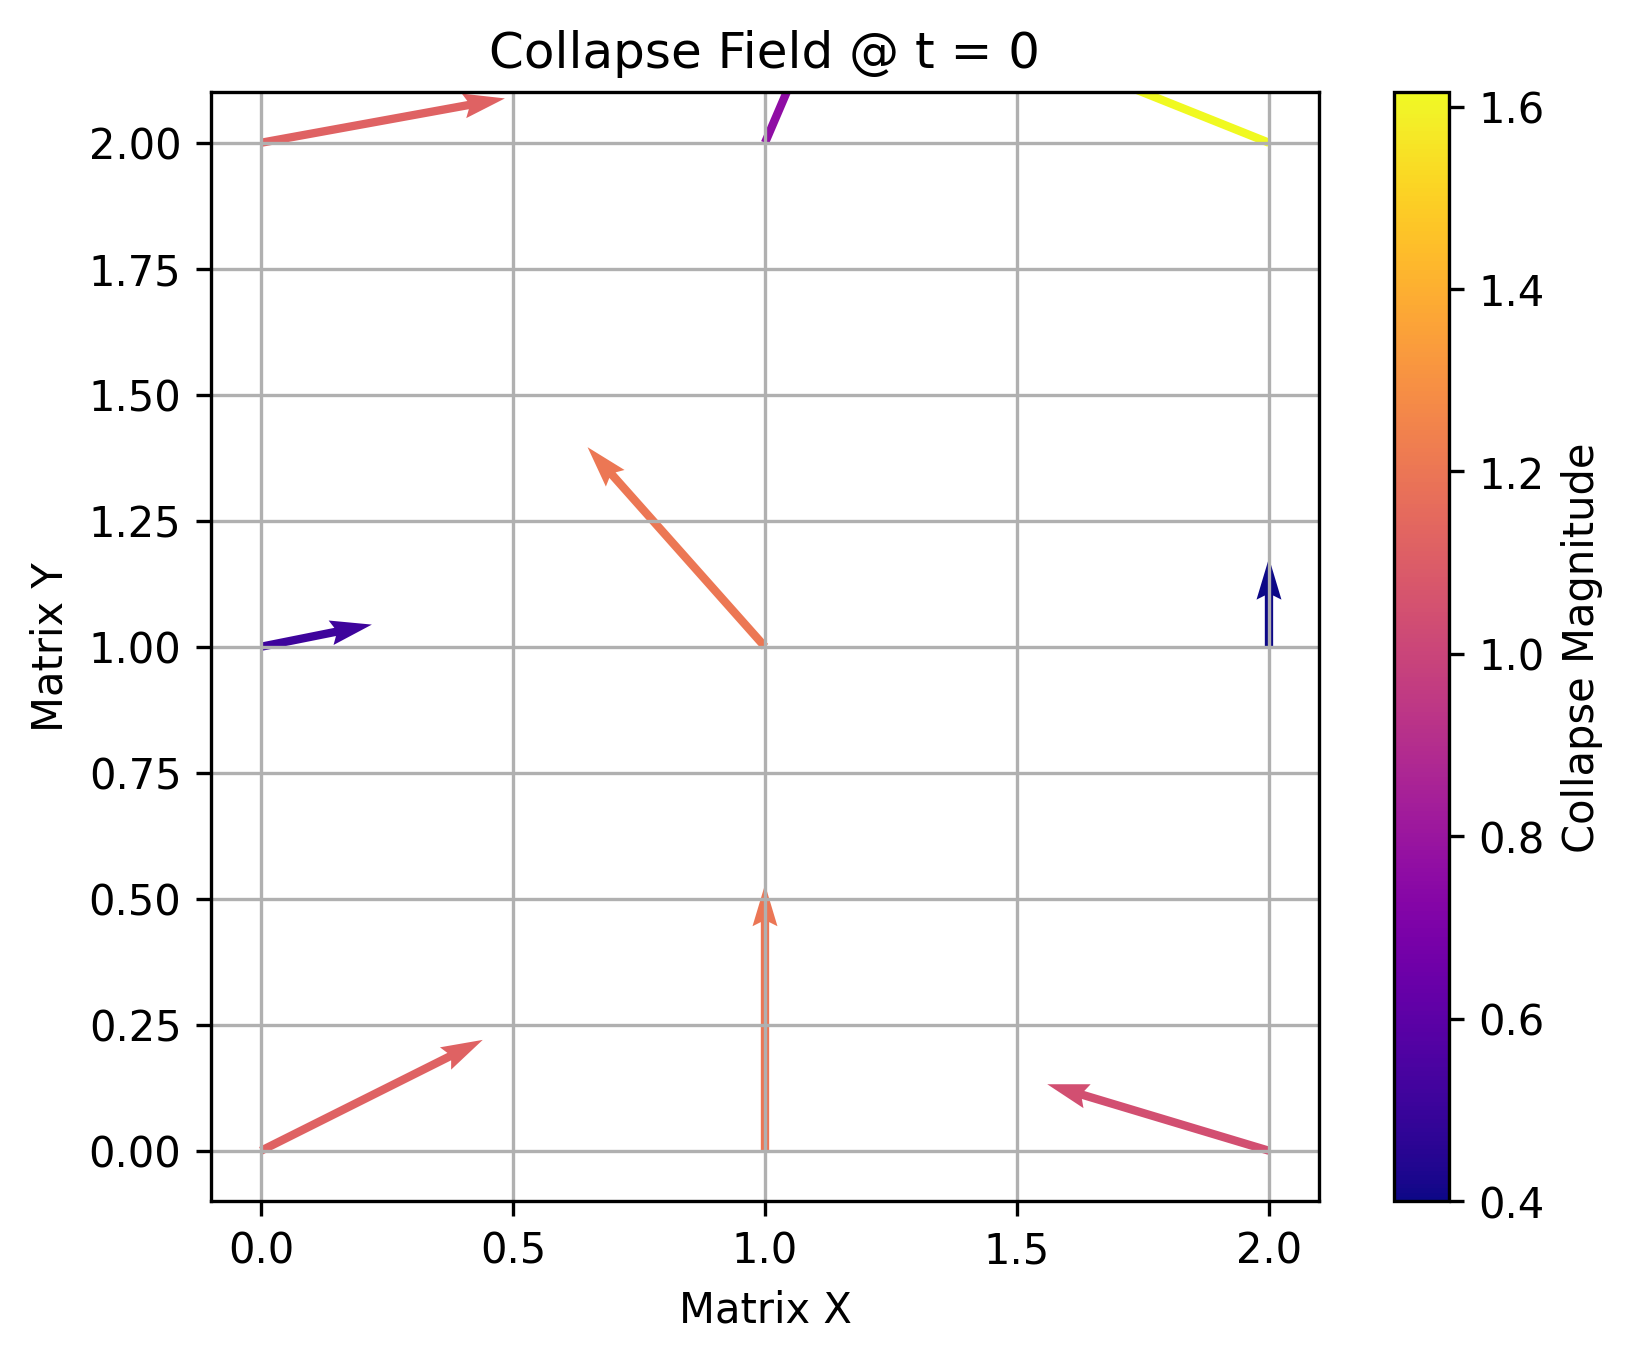
\includegraphics[width=\linewidth]{images/collapse_vector_t0.png}
      \caption{$t=0$ (Pre-collapse)}
    \end{subfigure}
    \hfill
    \begin{subfigure}[t]{0.3\textwidth}
      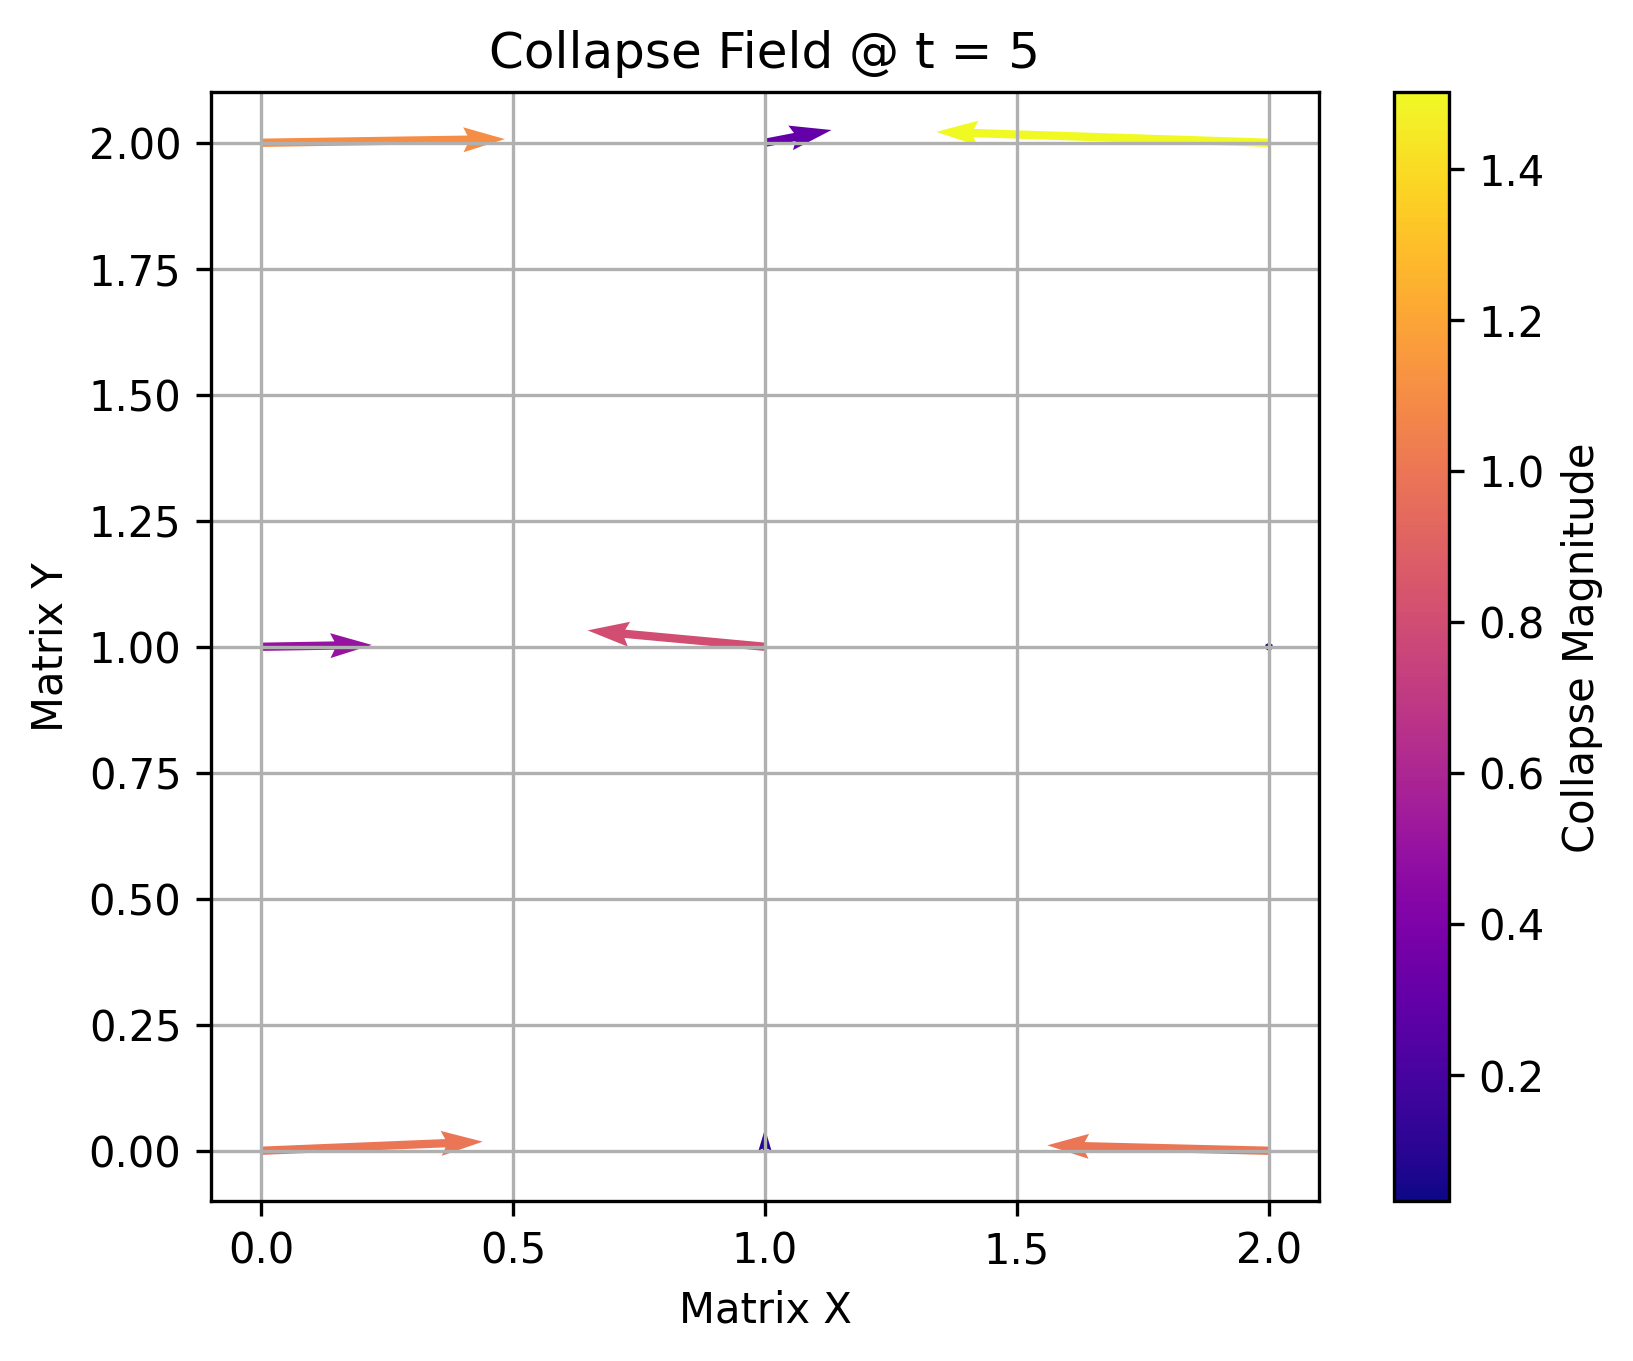
\includegraphics[width=\linewidth]{images/collapse_vector_t5.png}
      \caption{$t=5$ (Mid-collapse)}
    \end{subfigure}
    \hfill
    \begin{subfigure}[t]{0.3\textwidth}
      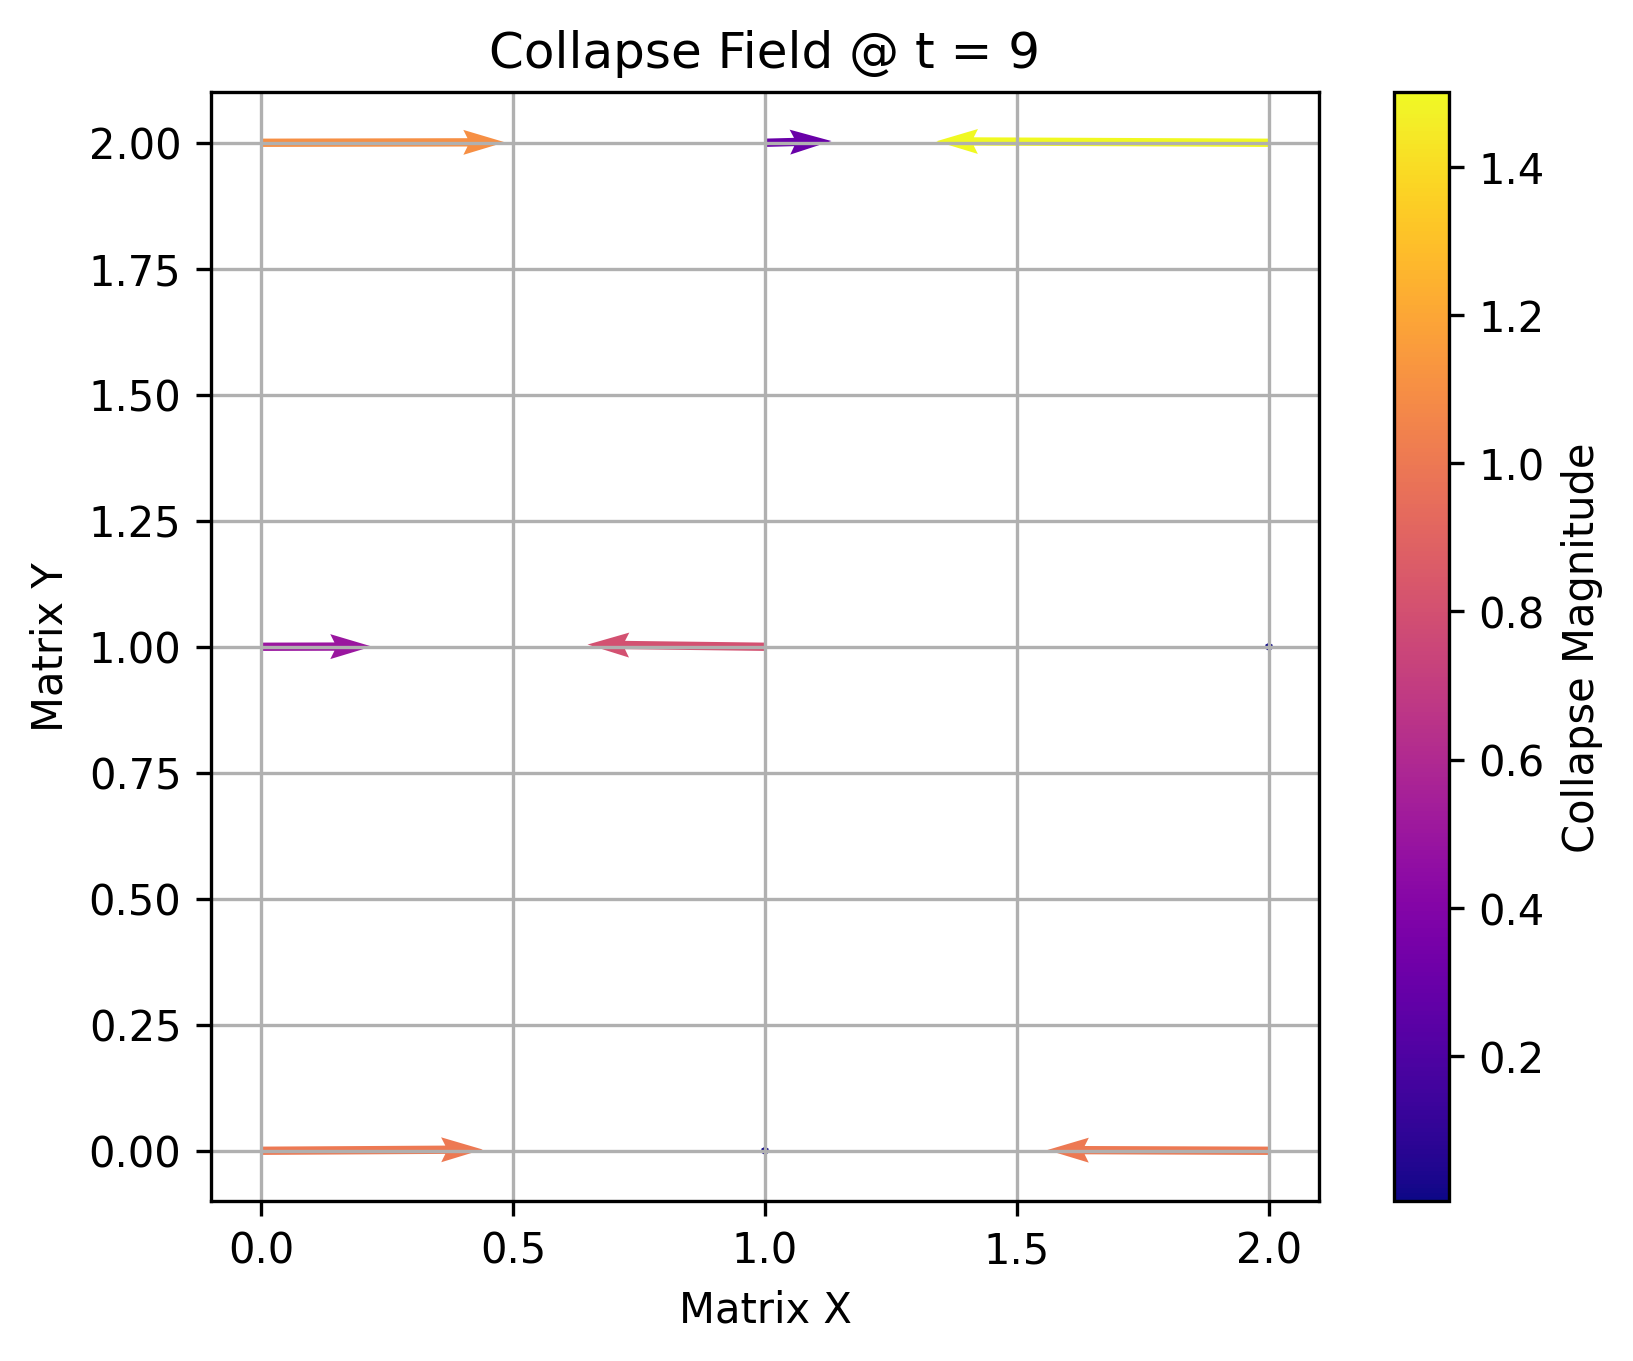
\includegraphics[width=\linewidth]{images/collapse_vector_t9.png}
      \caption{$t=9$ (Post-collapse)}
    \end{subfigure}
    \caption{Collapse vector field at three key stages. Imaginary potential collapses into resolved structure.}
    \label{fig:collapse_vector_series}
\end{figure}
  
\subsection*{Practical Framework for Visualization}



\begin{enumerate}
    \item \textbf{Data Preparation}:
    \begin{itemize}
        \item Construct a complex matrix $M = A + iB$ where $A$ and $B$ represent measurable and non-measurable states respectively. \cite{imaginary_meta} 
        \item Normalize the range of $A$ and $B$ to ensure visual coherence and relative continuity. 
    \end{itemize}

    \item \textbf{Decomposition}:
    \begin{itemize}
        \item Split $M$ into its real and imaginary components. 
        \item Assign $A$ to Z-coordinates or intensity values. 
        \item Assign $B$ to phase shifts, quiver directions, or color gradients. 
    \end{itemize}

    \item \textbf{Rendering Methodologies}:
    \begin{itemize}
        \item Voxel grid: Each voxel represents a matrix entry. Height = $a_{ij}$, color or vector rotation = $b_{ij}$. \cite{imaginary_meta} 
        \item Quiver plots: Vector fields showing directionality influenced by imaginary intensity. 
        \item Phase-encoded surfaces: Animate $B$ as a function of time or wave propagation. \cite{imaginary_meta} 
        \item Fourier mapping: Apply Fourier transforms to $M$ to reveal symmetry and spatial frequency. \cite{imaginary_meta} 
        \item Temporal layering: Render over iterations to create collapse-field time-lapse transitions. 
    \end{itemize}

    \item \textbf{Time Evolution}:
    \begin{itemize}
        \item Allow matrix values to evolve under a collapse simulation rule (e.g., damped wave equation or stochastic observation). \cite{imaginary_meta} 
        \item Track when $B \rightarrow 0$ as collapse finalizes into real projection, indicating completed observation. \cite{imaginary_meta} 
        \item Include visual boundaries to track entropic flow and decay rate. 
    \end{itemize}

    \item \textbf{Interpretation}:
    \begin{itemize}
        \item Identify stable attractor regions where $B$ diminishes predictably. 
        \item Mark chaotic regions where $B$ oscillates without coherence. 
        \item Visualize boundary zones where field resolution is actively occurring. 
        \item Extract localized field statistics for entropy, information density, and collapse gradient. \cite{imaginary_meta} 
      \end{itemize}
\end{enumerate}

\subsection*{Case Study: 3x3 Imaginary Matrix Collapse}

We construct a 3x3 complex matrix with real and imaginary parts:

\[
M =
\begin{bmatrix}
1 + i0.5 & 0 + i1.2 & -1 + i0.3 \\
0.5 + i0.1 & -0.8 + i0.9 & 0 + i0.4 \\
1.1 + i0.2 & 0.3 + i0.7 & -1.5 + i0.6
\end{bmatrix}
\]

\begin{itemize}
  \item \textbf{Initial Visualization:} Real matrix $A$ defines Z-height. \cite{imaginary_meta}
  \item Imaginary matrix $B$ defines hue.
  \item Each point represents a potential state pre-collapse. \cite{imaginary_meta}
  
  \item \textbf{Simulation:} Apply decay factor on $B$: $B(t+1) = B(t) \cdot e^{-\alpha t}$.
  
  \item \textbf{Observation:} Chaotic field vectors stabilize into $A$.
  \item Fourier transform reveals directionality.
  
  \item \textbf{Result:} Collapse to real structure. \cite{imaginary_meta}
  \item Dissipation of $B$.
\end{itemize}

\subsection{Imaginary Tensor Field Embedding in 3D Space}

\[
\mathcal{T}_{ij}(x, y, z, t) = A_{ij}(x, y, z) + iB_{ij}(x, y, z, t)
\]

Where:
\begin{itemize}
  \item $A_{ij}$ is the real symmetric tensor structure (observable classical deformation)
  \item $B_{ij}$ is the imaginary rotational component (collapse-phase curvature, time tension, or recursive flux)
\end{itemize}

These tensors can be visualized by:

\begin{itemize}
  \item Mapping \textbf{real components} to deformation (e.g., vector direction, surface normal)
  \item Mapping \textbf{imaginary components} to \textit{rotational shear}, hue, or curl-based motion vectors
  \item Encoding \textbf{tensor phase velocity} as:
\[
\omega_{ij}(x, t) = \frac{d}{dt} \arg(\mathcal{T}_{ij}) = \frac{\partial_t B_{ij}}{A_{ij}^2 + B_{ij}^2}
\]
\end{itemize}

This defines \textbf{phase rotation rates per tensor component}, providing a direct observable for imaginary field evolution. \cite{imaginary_meta} We treat $B_{ij}$ as defining a \textbf{local orthogonal tension field}---a vector shear axis that doesn’t exist in physical space, but influences real projections through:

\begin{itemize}
  \item Collapse stress
  \item Temporal quantization
  \item Observer-induced curvature
\end{itemize}

We further define a \textbf{Collapse Ricci Tensor} to represent second-order deformations sourced by imaginary curvature:

\[
\mathcal{R}^{(\text{collapse})}_{ij} = \nabla_i \nabla_j \left( \sqrt{A_{kl}A^{kl} + B_{kl}B^{kl}} \right)
\]

This construct reflects the curvature induced not by mass-energy, but by unresolved observation tension across the imaginary tensor field. \cite{imaginary_meta} As $B_{ij} \rightarrow 0$, the collapse Ricci converges to the curvature of the resolved real structure. \cite{imaginary_meta} When $B_{ij}$ dominates, $\mathcal{R}^{(\text{collapse})}_{ij}$ encodes \textit{imaginary pressure warping} that acts as precursor geometry. 

\subsubsection*{Visualization Strategy}
\begin{itemize}
  \item Plot \textbf{tensor ellipsoids} for $A_{ij}$
  \item Overlay rotational axes or vector fields from $B_{ij}$ as directional curls
  \item Use hue saturation or motion blur to encode imaginary rotation magnitude
  \item Compute trace and determinant over time to reveal collapse focal points and singularities
\end{itemize}

This renders the full Measurement Field as a \textbf{dual-reality system}: a visible classical domain with embedded imaginary-phase deformation, acting as the unseen architect of spacetime evolution. \cite{imaginary_meta} 

\subsubsection*{Applications of the Collapse Ricci Tensor}

The Collapse Ricci Tensor \( \mathcal{R}^{(\text{collapse})}_{ij} \) offers a new class of geometric observables for cosmological and quantum simulations. \cite{imaginary_meta} Beyond its theoretical value, it enables field diagnostics and simulation observables across multiple domains. 

\paragraph{Dark Energy Modeling}
Collapse curvature fields exhibit repulsive field tension. \cite{imaginary_meta} 

In zones of high imaginary tensor magnitude \( B_{ij} \), the divergence of \( \mathcal{R}^{(\text{collapse})}_{ij} \) yields an effective negative pressure:
\[
\nabla^i \mathcal{R}^{(\text{collapse})}_{ij} < 0 \quad \Rightarrow \quad \text{Local acceleration of spacetime separation}
\]
No cosmological constant is needed-dark energy arises from unresolved collapse tension. \cite{imaginary_meta} \paragraph{Pre-Collapse Structural Mapping}
Regions where \( \mathcal{R}^{(\text{collapse})} \) is high but \( A_{ij} \approx 0 \) are pre-collapse: proto-structures not yet resolved into classical form. \cite{imaginary_meta} These can be targeted in simulations and sky surveys as indicators of impending baryonic definition. \paragraph{Time Distortion Metrics}
High values of \( \mathcal{R}^{(\text{collapse})} \) directly influence the local collapse phase rate \( \omega_{ij} \), leading to dilated or looped time topologies:
\[
\frac{d\theta}{dt} \propto - \frac{B_{ij}}{A_{ij}^2 + B_{ij}^2} \quad \Rightarrow \quad \text{Temporal slowing where } B_{ij} \gg A_{ij}
\]

\paragraph{CMB Shell Deformation}
Implement \( \mathcal{R}^{(\text{collapse})} \) directly into HELLBLAST to deform spherical collapse projections. \cite{imaginary_meta} Use:
\[
\Delta T_{\ell m} \sim \int \mathcal{R}^{(\text{collapse})}_{ij} Y^*_{\ell m} \, d\Omega
\]
to model anisotropy and observer-relative collapse shells in the cosmic microwave background. \cite{imaginary_meta} \paragraph{Black Hole Boundary Geometry}
At collapse singularities, \( \mathcal{R}^{(\text{collapse})} \to \infty \). \cite{imaginary_meta} Define event horizon curvature through imaginary tension gradients:
\[\text{Surface gravity } \kappa \sim |\nabla B_{ij}|\]
Event horizons become zones of definitional collapse, not merely spacetime termination. \cite{imaginary_meta} \paragraph{Particle Decay Fields}
Spikes in \[ \mathcal{R}^{(\text{collapse})} \] may signal loss of phase stability or definitional coherence:

\[\mathcal{R}^{(\text{collapse})}_{ij} > \mathcal{R}_{\text{decay threshold}} \Rightarrow \text{Collapse instability} \Rightarrow \text{Particle decay}\]

This opens a predictive mechanism for decay events and quantum breakdowns. \cite{imaginary_meta} \paragraph{Simulation Engines (Lilith, Lucifer)}
Use \[ \mathcal{R}^{(\text{collapse})} \] as a procedural signal to define:
\begin{itemize}
  \item Collapse scars
  \item Time loops
  \item Observer boundary fluctuations
\end{itemize}

All of which drive emergent reality generation across simulated universes. \cite{imaginary_meta} \begin{center}
\textit{The Collapse Ricci Tensor is not a passive geometric structure. \cite{imaginary_meta} It is the definition-forcing curvature field of the Fifth Force-seen only in tension, resolved only through collapse.} \cite{imaginary_meta}
\end{center} 

\section*{Appendix A: Complete Citations for Chapter 1}

The following list contains all foundational works originally referenced during the construction of Chapter 1. These are preserved for rigor, despite being replaced with a condensed meta-citation in the body of the chapter.

\nocite{*}
\printbibliography[title={Appendix A References}, keyword=chapter1]
